\documentclass[border=5pt]{standalone}
\usepackage{tikz}
\usetikzlibrary{arrows.meta, positioning}
\usepackage{xcolor}

\definecolor{Garnet}{HTML}{73000A}
\definecolor{NinetyBlack}{HTML}{363636}
\definecolor{SeventyBlack}{HTML}{5C5C5C}
\definecolor{FiftyBlack}{HTML}{A2A2A2}
\definecolor{ThirtyBlack}{HTML}{C7C7C7}
\definecolor{TenBlack}{HTML}{ECECEC}
\definecolor{Atlantic}{HTML}{466A9F}
\definecolor{Sandstorm}{HTML}{FFF2E3}

\tikzset{every node/.append style={rounded corners=0pt}}

\begin{document}
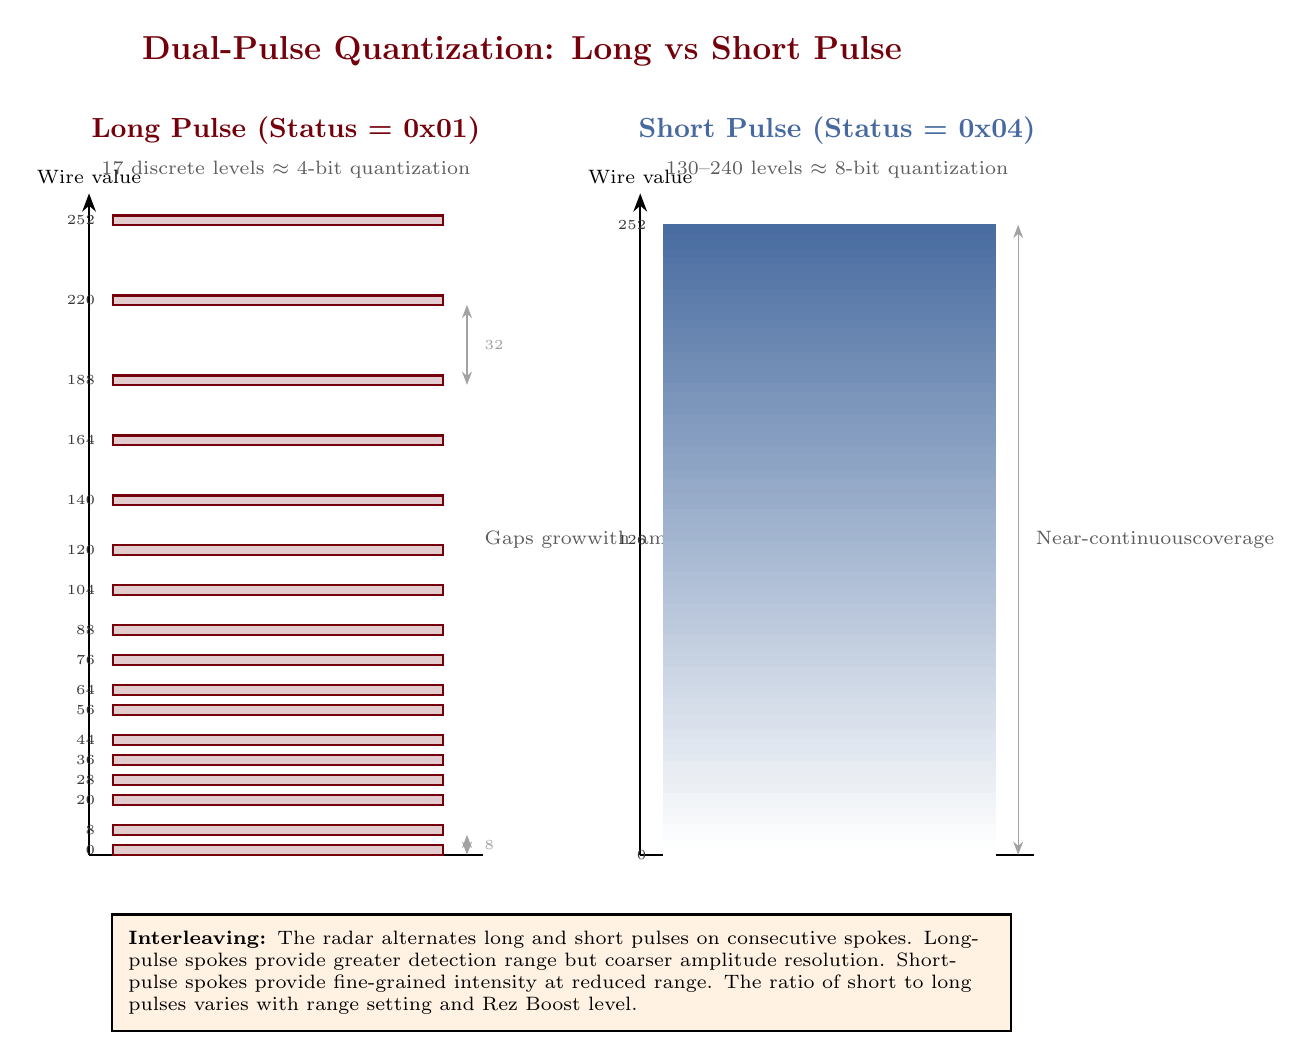
\begin{tikzpicture}[
    lbl/.style={font=\small\bfseries, color=NinetyBlack},
    annot/.style={font=\scriptsize, color=SeventyBlack},
]

\node[font=\bfseries\large, color=Garnet] at (5.5, 10.2) {Dual-Pulse Quantization: Long vs Short Pulse};

% ── Long Pulse (left) ──
\node[font=\bfseries, color=Garnet] at (2.5, 9.2) {Long Pulse (Status = 0x01)};
\node[annot] at (2.5, 8.7) {17 discrete levels $\approx$ 4-bit quantization};

% Y-axis
\draw[thick, -{Stealth}] (0, 0) -- (0, 8.4) node[above, font=\scriptsize] {Wire value};
% X-axis
\draw[thick] (0, 0) -- (5, 0);

% 17 discrete levels as horizontal bars
% Values: 0, 8, 20, 28, 36, 44, 56, 64, 76, 88, 104, 120, 140, 164, 188, 220, 252
% Scale: 252 -> 8.0, so multiply by 8/252 = 0.03175
\foreach \val/\y in {0/0, 8/0.254, 20/0.635, 28/0.889, 36/1.143, 44/1.397, 56/1.778, 64/2.032, 76/2.413, 88/2.794, 104/3.302, 120/3.810, 140/4.444, 164/5.206, 188/5.968, 220/6.984, 252/8.0} {
    \draw[thick, Garnet, fill=Garnet!20] (0.3, \y) rectangle (4.5, \y+0.12);
    \node[font=\tiny, color=NinetyBlack, anchor=east] at (0.2, \y+0.06) {\val};
}

% Gap annotations
\draw[{Stealth}-{Stealth}, thin, FiftyBlack] (4.8, 0) -- (4.8, 0.254);
\draw[{Stealth}-{Stealth}, thin, FiftyBlack] (4.8, 5.968) -- (4.8, 6.984);
\node[font=\tiny, color=FiftyBlack, anchor=west] at (4.9, 0.127) {8};
\node[font=\tiny, color=FiftyBlack, anchor=west] at (4.9, 6.476) {32};
\node[annot, anchor=west] at (4.9, 4.0) {Gaps grow\\with amplitude};

% ── Short Pulse (right) ──
\node[font=\bfseries, color=Atlantic] at (9.5, 9.2) {Short Pulse (Status = 0x04)};
\node[annot] at (9.5, 8.7) {130--240 levels $\approx$ 8-bit quantization};

% Y-axis
\draw[thick, -{Stealth}] (7, 0) -- (7, 8.4) node[above, font=\scriptsize] {Wire value};
% X-axis
\draw[thick] (7, 0) -- (12, 0);

% Continuous gradient (simulated with many thin bars)
\foreach \i in {0,1,...,79} {
    \pgfmathsetmacro{\ypos}{\i * 0.1}
    \pgfmathsetmacro{\intensity}{int(\i * 100 / 80)}
    \draw[thick, Atlantic!\intensity!white, fill=Atlantic!\intensity!white] (7.3, \ypos) rectangle (11.5, \ypos+0.1);
}

% Scale labels
\node[font=\tiny, color=NinetyBlack, anchor=east] at (7.2, 0) {0};
\node[font=\tiny, color=NinetyBlack, anchor=east] at (7.2, 4.0) {126};
\node[font=\tiny, color=NinetyBlack, anchor=east] at (7.2, 8.0) {252};

% Continuous annotation
\draw[{Stealth}-{Stealth}, thin, FiftyBlack] (11.8, 0) -- (11.8, 8.0);
\node[annot, anchor=west] at (11.9, 4.0) {Near-continuous\\coverage};

% ── Comparison note ──
\node[draw, thick, fill=Sandstorm, text width=11cm, align=left, font=\scriptsize, inner sep=6pt] at (6, -1.5) {
\textbf{Interleaving:} The radar alternates long and short pulses on consecutive spokes. Long-pulse spokes provide greater detection range but coarser amplitude resolution. Short-pulse spokes provide fine-grained intensity at reduced range. The ratio of short to long pulses varies with range setting and Rez Boost level.
};

\end{tikzpicture}
\end{document}
